
% Default to the notebook output style

    


% Inherit from the specified cell style.




    
\documentclass[11pt]{article}

    
    
    \usepackage[T1]{fontenc}
    % Nicer default font (+ math font) than Computer Modern for most use cases
    \usepackage{mathpazo}

    % Basic figure setup, for now with no caption control since it's done
    % automatically by Pandoc (which extracts ![](path) syntax from Markdown).
    \usepackage{graphicx}
    % We will generate all images so they have a width \maxwidth. This means
    % that they will get their normal width if they fit onto the page, but
    % are scaled down if they would overflow the margins.
    \makeatletter
    \def\maxwidth{\ifdim\Gin@nat@width>\linewidth\linewidth
    \else\Gin@nat@width\fi}
    \makeatother
    \let\Oldincludegraphics\includegraphics
    % Set max figure width to be 80% of text width, for now hardcoded.
    \renewcommand{\includegraphics}[1]{\Oldincludegraphics[width=.8\maxwidth]{#1}}
    % Ensure that by default, figures have no caption (until we provide a
    % proper Figure object with a Caption API and a way to capture that
    % in the conversion process - todo).
    \usepackage{caption}
    \DeclareCaptionLabelFormat{nolabel}{}
    \captionsetup{labelformat=nolabel}

    \usepackage{adjustbox} % Used to constrain images to a maximum size 
    \usepackage{xcolor} % Allow colors to be defined
    \usepackage{enumerate} % Needed for markdown enumerations to work
    \usepackage{geometry} % Used to adjust the document margins
    \usepackage{amsmath} % Equations
    \usepackage{amssymb} % Equations
    \usepackage{textcomp} % defines textquotesingle
    % Hack from http://tex.stackexchange.com/a/47451/13684:
    \AtBeginDocument{%
        \def\PYZsq{\textquotesingle}% Upright quotes in Pygmentized code
    }
    \usepackage{upquote} % Upright quotes for verbatim code
    \usepackage{eurosym} % defines \euro
    \usepackage[mathletters]{ucs} % Extended unicode (utf-8) support
    \usepackage[utf8x]{inputenc} % Allow utf-8 characters in the tex document
    \usepackage{fancyvrb} % verbatim replacement that allows latex
    \usepackage{grffile} % extends the file name processing of package graphics 
                         % to support a larger range 
    % The hyperref package gives us a pdf with properly built
    % internal navigation ('pdf bookmarks' for the table of contents,
    % internal cross-reference links, web links for URLs, etc.)
    \usepackage{hyperref}
    \usepackage{longtable} % longtable support required by pandoc >1.10
    \usepackage{booktabs}  % table support for pandoc > 1.12.2
    \usepackage[inline]{enumitem} % IRkernel/repr support (it uses the enumerate* environment)
    \usepackage[normalem]{ulem} % ulem is needed to support strikethroughs (\sout)
                                % normalem makes italics be italics, not underlines
    

    
    
    % Colors for the hyperref package
    \definecolor{urlcolor}{rgb}{0,.145,.698}
    \definecolor{linkcolor}{rgb}{.71,0.21,0.01}
    \definecolor{citecolor}{rgb}{.12,.54,.11}

    % ANSI colors
    \definecolor{ansi-black}{HTML}{3E424D}
    \definecolor{ansi-black-intense}{HTML}{282C36}
    \definecolor{ansi-red}{HTML}{E75C58}
    \definecolor{ansi-red-intense}{HTML}{B22B31}
    \definecolor{ansi-green}{HTML}{00A250}
    \definecolor{ansi-green-intense}{HTML}{007427}
    \definecolor{ansi-yellow}{HTML}{DDB62B}
    \definecolor{ansi-yellow-intense}{HTML}{B27D12}
    \definecolor{ansi-blue}{HTML}{208FFB}
    \definecolor{ansi-blue-intense}{HTML}{0065CA}
    \definecolor{ansi-magenta}{HTML}{D160C4}
    \definecolor{ansi-magenta-intense}{HTML}{A03196}
    \definecolor{ansi-cyan}{HTML}{60C6C8}
    \definecolor{ansi-cyan-intense}{HTML}{258F8F}
    \definecolor{ansi-white}{HTML}{C5C1B4}
    \definecolor{ansi-white-intense}{HTML}{A1A6B2}

    % commands and environments needed by pandoc snippets
    % extracted from the output of `pandoc -s`
    \providecommand{\tightlist}{%
      \setlength{\itemsep}{0pt}\setlength{\parskip}{0pt}}
    \DefineVerbatimEnvironment{Highlighting}{Verbatim}{commandchars=\\\{\}}
    % Add ',fontsize=\small' for more characters per line
    \newenvironment{Shaded}{}{}
    \newcommand{\KeywordTok}[1]{\textcolor[rgb]{0.00,0.44,0.13}{\textbf{{#1}}}}
    \newcommand{\DataTypeTok}[1]{\textcolor[rgb]{0.56,0.13,0.00}{{#1}}}
    \newcommand{\DecValTok}[1]{\textcolor[rgb]{0.25,0.63,0.44}{{#1}}}
    \newcommand{\BaseNTok}[1]{\textcolor[rgb]{0.25,0.63,0.44}{{#1}}}
    \newcommand{\FloatTok}[1]{\textcolor[rgb]{0.25,0.63,0.44}{{#1}}}
    \newcommand{\CharTok}[1]{\textcolor[rgb]{0.25,0.44,0.63}{{#1}}}
    \newcommand{\StringTok}[1]{\textcolor[rgb]{0.25,0.44,0.63}{{#1}}}
    \newcommand{\CommentTok}[1]{\textcolor[rgb]{0.38,0.63,0.69}{\textit{{#1}}}}
    \newcommand{\OtherTok}[1]{\textcolor[rgb]{0.00,0.44,0.13}{{#1}}}
    \newcommand{\AlertTok}[1]{\textcolor[rgb]{1.00,0.00,0.00}{\textbf{{#1}}}}
    \newcommand{\FunctionTok}[1]{\textcolor[rgb]{0.02,0.16,0.49}{{#1}}}
    \newcommand{\RegionMarkerTok}[1]{{#1}}
    \newcommand{\ErrorTok}[1]{\textcolor[rgb]{1.00,0.00,0.00}{\textbf{{#1}}}}
    \newcommand{\NormalTok}[1]{{#1}}
    
    % Additional commands for more recent versions of Pandoc
    \newcommand{\ConstantTok}[1]{\textcolor[rgb]{0.53,0.00,0.00}{{#1}}}
    \newcommand{\SpecialCharTok}[1]{\textcolor[rgb]{0.25,0.44,0.63}{{#1}}}
    \newcommand{\VerbatimStringTok}[1]{\textcolor[rgb]{0.25,0.44,0.63}{{#1}}}
    \newcommand{\SpecialStringTok}[1]{\textcolor[rgb]{0.73,0.40,0.53}{{#1}}}
    \newcommand{\ImportTok}[1]{{#1}}
    \newcommand{\DocumentationTok}[1]{\textcolor[rgb]{0.73,0.13,0.13}{\textit{{#1}}}}
    \newcommand{\AnnotationTok}[1]{\textcolor[rgb]{0.38,0.63,0.69}{\textbf{\textit{{#1}}}}}
    \newcommand{\CommentVarTok}[1]{\textcolor[rgb]{0.38,0.63,0.69}{\textbf{\textit{{#1}}}}}
    \newcommand{\VariableTok}[1]{\textcolor[rgb]{0.10,0.09,0.49}{{#1}}}
    \newcommand{\ControlFlowTok}[1]{\textcolor[rgb]{0.00,0.44,0.13}{\textbf{{#1}}}}
    \newcommand{\OperatorTok}[1]{\textcolor[rgb]{0.40,0.40,0.40}{{#1}}}
    \newcommand{\BuiltInTok}[1]{{#1}}
    \newcommand{\ExtensionTok}[1]{{#1}}
    \newcommand{\PreprocessorTok}[1]{\textcolor[rgb]{0.74,0.48,0.00}{{#1}}}
    \newcommand{\AttributeTok}[1]{\textcolor[rgb]{0.49,0.56,0.16}{{#1}}}
    \newcommand{\InformationTok}[1]{\textcolor[rgb]{0.38,0.63,0.69}{\textbf{\textit{{#1}}}}}
    \newcommand{\WarningTok}[1]{\textcolor[rgb]{0.38,0.63,0.69}{\textbf{\textit{{#1}}}}}
    
    
    % Define a nice break command that doesn't care if a line doesn't already
    % exist.
    \def\br{\hspace*{\fill} \\* }
    % Math Jax compatability definitions
    \def\gt{>}
    \def\lt{<}
    % Document parameters
    \title{Tutorial\_Session2}
    
    
    

    % Pygments definitions
    
\makeatletter
\def\PY@reset{\let\PY@it=\relax \let\PY@bf=\relax%
    \let\PY@ul=\relax \let\PY@tc=\relax%
    \let\PY@bc=\relax \let\PY@ff=\relax}
\def\PY@tok#1{\csname PY@tok@#1\endcsname}
\def\PY@toks#1+{\ifx\relax#1\empty\else%
    \PY@tok{#1}\expandafter\PY@toks\fi}
\def\PY@do#1{\PY@bc{\PY@tc{\PY@ul{%
    \PY@it{\PY@bf{\PY@ff{#1}}}}}}}
\def\PY#1#2{\PY@reset\PY@toks#1+\relax+\PY@do{#2}}

\expandafter\def\csname PY@tok@w\endcsname{\def\PY@tc##1{\textcolor[rgb]{0.73,0.73,0.73}{##1}}}
\expandafter\def\csname PY@tok@c\endcsname{\let\PY@it=\textit\def\PY@tc##1{\textcolor[rgb]{0.25,0.50,0.50}{##1}}}
\expandafter\def\csname PY@tok@cp\endcsname{\def\PY@tc##1{\textcolor[rgb]{0.74,0.48,0.00}{##1}}}
\expandafter\def\csname PY@tok@k\endcsname{\let\PY@bf=\textbf\def\PY@tc##1{\textcolor[rgb]{0.00,0.50,0.00}{##1}}}
\expandafter\def\csname PY@tok@kp\endcsname{\def\PY@tc##1{\textcolor[rgb]{0.00,0.50,0.00}{##1}}}
\expandafter\def\csname PY@tok@kt\endcsname{\def\PY@tc##1{\textcolor[rgb]{0.69,0.00,0.25}{##1}}}
\expandafter\def\csname PY@tok@o\endcsname{\def\PY@tc##1{\textcolor[rgb]{0.40,0.40,0.40}{##1}}}
\expandafter\def\csname PY@tok@ow\endcsname{\let\PY@bf=\textbf\def\PY@tc##1{\textcolor[rgb]{0.67,0.13,1.00}{##1}}}
\expandafter\def\csname PY@tok@nb\endcsname{\def\PY@tc##1{\textcolor[rgb]{0.00,0.50,0.00}{##1}}}
\expandafter\def\csname PY@tok@nf\endcsname{\def\PY@tc##1{\textcolor[rgb]{0.00,0.00,1.00}{##1}}}
\expandafter\def\csname PY@tok@nc\endcsname{\let\PY@bf=\textbf\def\PY@tc##1{\textcolor[rgb]{0.00,0.00,1.00}{##1}}}
\expandafter\def\csname PY@tok@nn\endcsname{\let\PY@bf=\textbf\def\PY@tc##1{\textcolor[rgb]{0.00,0.00,1.00}{##1}}}
\expandafter\def\csname PY@tok@ne\endcsname{\let\PY@bf=\textbf\def\PY@tc##1{\textcolor[rgb]{0.82,0.25,0.23}{##1}}}
\expandafter\def\csname PY@tok@nv\endcsname{\def\PY@tc##1{\textcolor[rgb]{0.10,0.09,0.49}{##1}}}
\expandafter\def\csname PY@tok@no\endcsname{\def\PY@tc##1{\textcolor[rgb]{0.53,0.00,0.00}{##1}}}
\expandafter\def\csname PY@tok@nl\endcsname{\def\PY@tc##1{\textcolor[rgb]{0.63,0.63,0.00}{##1}}}
\expandafter\def\csname PY@tok@ni\endcsname{\let\PY@bf=\textbf\def\PY@tc##1{\textcolor[rgb]{0.60,0.60,0.60}{##1}}}
\expandafter\def\csname PY@tok@na\endcsname{\def\PY@tc##1{\textcolor[rgb]{0.49,0.56,0.16}{##1}}}
\expandafter\def\csname PY@tok@nt\endcsname{\let\PY@bf=\textbf\def\PY@tc##1{\textcolor[rgb]{0.00,0.50,0.00}{##1}}}
\expandafter\def\csname PY@tok@nd\endcsname{\def\PY@tc##1{\textcolor[rgb]{0.67,0.13,1.00}{##1}}}
\expandafter\def\csname PY@tok@s\endcsname{\def\PY@tc##1{\textcolor[rgb]{0.73,0.13,0.13}{##1}}}
\expandafter\def\csname PY@tok@sd\endcsname{\let\PY@it=\textit\def\PY@tc##1{\textcolor[rgb]{0.73,0.13,0.13}{##1}}}
\expandafter\def\csname PY@tok@si\endcsname{\let\PY@bf=\textbf\def\PY@tc##1{\textcolor[rgb]{0.73,0.40,0.53}{##1}}}
\expandafter\def\csname PY@tok@se\endcsname{\let\PY@bf=\textbf\def\PY@tc##1{\textcolor[rgb]{0.73,0.40,0.13}{##1}}}
\expandafter\def\csname PY@tok@sr\endcsname{\def\PY@tc##1{\textcolor[rgb]{0.73,0.40,0.53}{##1}}}
\expandafter\def\csname PY@tok@ss\endcsname{\def\PY@tc##1{\textcolor[rgb]{0.10,0.09,0.49}{##1}}}
\expandafter\def\csname PY@tok@sx\endcsname{\def\PY@tc##1{\textcolor[rgb]{0.00,0.50,0.00}{##1}}}
\expandafter\def\csname PY@tok@m\endcsname{\def\PY@tc##1{\textcolor[rgb]{0.40,0.40,0.40}{##1}}}
\expandafter\def\csname PY@tok@gh\endcsname{\let\PY@bf=\textbf\def\PY@tc##1{\textcolor[rgb]{0.00,0.00,0.50}{##1}}}
\expandafter\def\csname PY@tok@gu\endcsname{\let\PY@bf=\textbf\def\PY@tc##1{\textcolor[rgb]{0.50,0.00,0.50}{##1}}}
\expandafter\def\csname PY@tok@gd\endcsname{\def\PY@tc##1{\textcolor[rgb]{0.63,0.00,0.00}{##1}}}
\expandafter\def\csname PY@tok@gi\endcsname{\def\PY@tc##1{\textcolor[rgb]{0.00,0.63,0.00}{##1}}}
\expandafter\def\csname PY@tok@gr\endcsname{\def\PY@tc##1{\textcolor[rgb]{1.00,0.00,0.00}{##1}}}
\expandafter\def\csname PY@tok@ge\endcsname{\let\PY@it=\textit}
\expandafter\def\csname PY@tok@gs\endcsname{\let\PY@bf=\textbf}
\expandafter\def\csname PY@tok@gp\endcsname{\let\PY@bf=\textbf\def\PY@tc##1{\textcolor[rgb]{0.00,0.00,0.50}{##1}}}
\expandafter\def\csname PY@tok@go\endcsname{\def\PY@tc##1{\textcolor[rgb]{0.53,0.53,0.53}{##1}}}
\expandafter\def\csname PY@tok@gt\endcsname{\def\PY@tc##1{\textcolor[rgb]{0.00,0.27,0.87}{##1}}}
\expandafter\def\csname PY@tok@err\endcsname{\def\PY@bc##1{\setlength{\fboxsep}{0pt}\fcolorbox[rgb]{1.00,0.00,0.00}{1,1,1}{\strut ##1}}}
\expandafter\def\csname PY@tok@kc\endcsname{\let\PY@bf=\textbf\def\PY@tc##1{\textcolor[rgb]{0.00,0.50,0.00}{##1}}}
\expandafter\def\csname PY@tok@kd\endcsname{\let\PY@bf=\textbf\def\PY@tc##1{\textcolor[rgb]{0.00,0.50,0.00}{##1}}}
\expandafter\def\csname PY@tok@kn\endcsname{\let\PY@bf=\textbf\def\PY@tc##1{\textcolor[rgb]{0.00,0.50,0.00}{##1}}}
\expandafter\def\csname PY@tok@kr\endcsname{\let\PY@bf=\textbf\def\PY@tc##1{\textcolor[rgb]{0.00,0.50,0.00}{##1}}}
\expandafter\def\csname PY@tok@bp\endcsname{\def\PY@tc##1{\textcolor[rgb]{0.00,0.50,0.00}{##1}}}
\expandafter\def\csname PY@tok@fm\endcsname{\def\PY@tc##1{\textcolor[rgb]{0.00,0.00,1.00}{##1}}}
\expandafter\def\csname PY@tok@vc\endcsname{\def\PY@tc##1{\textcolor[rgb]{0.10,0.09,0.49}{##1}}}
\expandafter\def\csname PY@tok@vg\endcsname{\def\PY@tc##1{\textcolor[rgb]{0.10,0.09,0.49}{##1}}}
\expandafter\def\csname PY@tok@vi\endcsname{\def\PY@tc##1{\textcolor[rgb]{0.10,0.09,0.49}{##1}}}
\expandafter\def\csname PY@tok@vm\endcsname{\def\PY@tc##1{\textcolor[rgb]{0.10,0.09,0.49}{##1}}}
\expandafter\def\csname PY@tok@sa\endcsname{\def\PY@tc##1{\textcolor[rgb]{0.73,0.13,0.13}{##1}}}
\expandafter\def\csname PY@tok@sb\endcsname{\def\PY@tc##1{\textcolor[rgb]{0.73,0.13,0.13}{##1}}}
\expandafter\def\csname PY@tok@sc\endcsname{\def\PY@tc##1{\textcolor[rgb]{0.73,0.13,0.13}{##1}}}
\expandafter\def\csname PY@tok@dl\endcsname{\def\PY@tc##1{\textcolor[rgb]{0.73,0.13,0.13}{##1}}}
\expandafter\def\csname PY@tok@s2\endcsname{\def\PY@tc##1{\textcolor[rgb]{0.73,0.13,0.13}{##1}}}
\expandafter\def\csname PY@tok@sh\endcsname{\def\PY@tc##1{\textcolor[rgb]{0.73,0.13,0.13}{##1}}}
\expandafter\def\csname PY@tok@s1\endcsname{\def\PY@tc##1{\textcolor[rgb]{0.73,0.13,0.13}{##1}}}
\expandafter\def\csname PY@tok@mb\endcsname{\def\PY@tc##1{\textcolor[rgb]{0.40,0.40,0.40}{##1}}}
\expandafter\def\csname PY@tok@mf\endcsname{\def\PY@tc##1{\textcolor[rgb]{0.40,0.40,0.40}{##1}}}
\expandafter\def\csname PY@tok@mh\endcsname{\def\PY@tc##1{\textcolor[rgb]{0.40,0.40,0.40}{##1}}}
\expandafter\def\csname PY@tok@mi\endcsname{\def\PY@tc##1{\textcolor[rgb]{0.40,0.40,0.40}{##1}}}
\expandafter\def\csname PY@tok@il\endcsname{\def\PY@tc##1{\textcolor[rgb]{0.40,0.40,0.40}{##1}}}
\expandafter\def\csname PY@tok@mo\endcsname{\def\PY@tc##1{\textcolor[rgb]{0.40,0.40,0.40}{##1}}}
\expandafter\def\csname PY@tok@ch\endcsname{\let\PY@it=\textit\def\PY@tc##1{\textcolor[rgb]{0.25,0.50,0.50}{##1}}}
\expandafter\def\csname PY@tok@cm\endcsname{\let\PY@it=\textit\def\PY@tc##1{\textcolor[rgb]{0.25,0.50,0.50}{##1}}}
\expandafter\def\csname PY@tok@cpf\endcsname{\let\PY@it=\textit\def\PY@tc##1{\textcolor[rgb]{0.25,0.50,0.50}{##1}}}
\expandafter\def\csname PY@tok@c1\endcsname{\let\PY@it=\textit\def\PY@tc##1{\textcolor[rgb]{0.25,0.50,0.50}{##1}}}
\expandafter\def\csname PY@tok@cs\endcsname{\let\PY@it=\textit\def\PY@tc##1{\textcolor[rgb]{0.25,0.50,0.50}{##1}}}

\def\PYZbs{\char`\\}
\def\PYZus{\char`\_}
\def\PYZob{\char`\{}
\def\PYZcb{\char`\}}
\def\PYZca{\char`\^}
\def\PYZam{\char`\&}
\def\PYZlt{\char`\<}
\def\PYZgt{\char`\>}
\def\PYZsh{\char`\#}
\def\PYZpc{\char`\%}
\def\PYZdl{\char`\$}
\def\PYZhy{\char`\-}
\def\PYZsq{\char`\'}
\def\PYZdq{\char`\"}
\def\PYZti{\char`\~}
% for compatibility with earlier versions
\def\PYZat{@}
\def\PYZlb{[}
\def\PYZrb{]}
\makeatother


    % Exact colors from NB
    \definecolor{incolor}{rgb}{0.0, 0.0, 0.5}
    \definecolor{outcolor}{rgb}{0.545, 0.0, 0.0}



    
    % Prevent overflowing lines due to hard-to-break entities
    \sloppy 
    % Setup hyperref package
    \hypersetup{
      breaklinks=true,  % so long urls are correctly broken across lines
      colorlinks=true,
      urlcolor=urlcolor,
      linkcolor=linkcolor,
      citecolor=citecolor,
      }
    % Slightly bigger margins than the latex defaults
    
    \geometry{verbose,tmargin=1in,bmargin=1in,lmargin=1in,rmargin=1in}
    
    

    \begin{document}
    
    
    \maketitle
    
    

    
    \section{String and List}\label{string-and-list}

    \subsection{ Strings }\label{strings}

\begin{itemize}
\tightlist
\item
  A string is a sequence of characters.
\item
  A string may be specified by placing the member characters of the
  sequence within quotes (single, double or triple).
\item
  Triple quotes are typically used for strings that span multiple lines.
\end{itemize}

    \begin{Verbatim}[commandchars=\\\{\}]
{\color{incolor}In [{\color{incolor}1}]:} \PY{n}{message} \PY{o}{=} \PY{l+s+s1}{\PYZsq{}}\PY{l+s+s1}{Hello Gita}\PY{l+s+s1}{\PYZsq{}}
\end{Verbatim}


    \subsubsection{ Computing Length using len function
}\label{computing-length-using-len-function}

    \begin{Verbatim}[commandchars=\\\{\}]
{\color{incolor}In [{\color{incolor}2}]:} \PY{n+nb}{print}\PY{p}{(}\PY{n+nb}{len}\PY{p}{(}\PY{n}{message}\PY{p}{)}\PY{p}{)}
\end{Verbatim}


    \begin{Verbatim}[commandchars=\\\{\}]
10

    \end{Verbatim}

    \subsubsection{ Indexing }\label{indexing}

\begin{itemize}
\tightlist
\item
  Individual characters within a string are accessed using a technique
  known as indexing.

  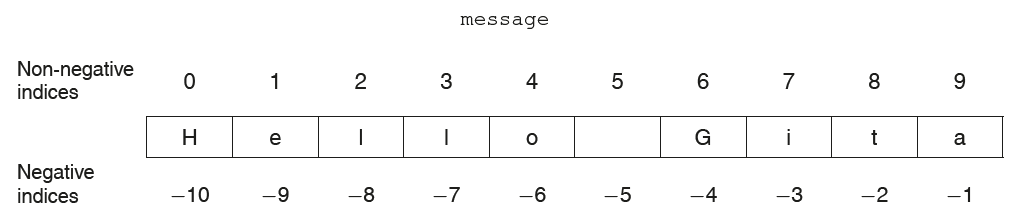
\includegraphics{1.png}
\end{itemize}

    \begin{Verbatim}[commandchars=\\\{\}]
{\color{incolor}In [{\color{incolor}3}]:} \PY{n}{index} \PY{o}{=} \PY{n+nb}{len}\PY{p}{(}\PY{n}{message}\PY{p}{)} \PY{o}{\PYZhy{}} \PY{l+m+mi}{1}
        \PY{n+nb}{print}\PY{p}{(}\PY{n}{message}\PY{p}{[}\PY{l+m+mi}{0}\PY{p}{]}\PY{p}{,} \PY{n}{message}\PY{p}{[}\PY{l+m+mi}{6}\PY{p}{]}\PY{p}{,} \PY{n}{message}\PY{p}{[}\PY{n}{index}\PY{p}{]}\PY{p}{,} \PY{n}{message}\PY{p}{[}\PY{o}{\PYZhy{}}\PY{l+m+mi}{1}\PY{p}{]}\PY{p}{)}
\end{Verbatim}


    \begin{Verbatim}[commandchars=\\\{\}]
H G a a

    \end{Verbatim}

    \begin{Verbatim}[commandchars=\\\{\}]
{\color{incolor}In [{\color{incolor}4}]:} \PY{n+nb}{print}\PY{p}{(}\PY{n}{message}\PY{p}{[}\PY{l+m+mi}{15}\PY{p}{]}\PY{p}{)}
\end{Verbatim}


    \begin{Verbatim}[commandchars=\\\{\}]

        ---------------------------------------------------------------------------

        IndexError                                Traceback (most recent call last)

        <ipython-input-4-a801df50d8d1> in <module>()
    ----> 1 print(message[15])
    

        IndexError: string index out of range

    \end{Verbatim}

    \subsubsection{ Slicing }\label{slicing}

\begin{itemize}
\tightlist
\item
  In order to extract the substring comprising the character sequence
  having indices from start to end-1, we specify the range in the form
  start:end.
\item
  Python also allows us to extract a subsequence of the form
  \emph{start:end:inc}.
\end{itemize}

    \begin{Verbatim}[commandchars=\\\{\}]
{\color{incolor}In [{\color{incolor}89}]:} \PY{n}{message} \PY{o}{=} \PY{l+s+s1}{\PYZsq{}}\PY{l+s+s1}{Hello Sita}\PY{l+s+s1}{\PYZsq{}}
         \PY{n+nb}{print}\PY{p}{(}\PY{n}{message}\PY{p}{[}\PY{l+m+mi}{0}\PY{p}{:}\PY{l+m+mi}{5}\PY{p}{]}\PY{p}{,} \PY{n}{message}\PY{p}{[}\PY{o}{\PYZhy{}}\PY{l+m+mi}{10}\PY{p}{:}\PY{o}{\PYZhy{}}\PY{l+m+mi}{5}\PY{p}{]}\PY{p}{)}
\end{Verbatim}


    \begin{Verbatim}[commandchars=\\\{\}]
Hello Hello

    \end{Verbatim}

    \begin{Verbatim}[commandchars=\\\{\}]
{\color{incolor}In [{\color{incolor}90}]:} \PY{n+nb}{print}\PY{p}{(}\PY{n}{message}\PY{p}{[}\PY{l+m+mi}{0}\PY{p}{:}\PY{n+nb}{len}\PY{p}{(}\PY{n}{message}\PY{p}{)}\PY{p}{:}\PY{l+m+mi}{2}\PY{p}{]}\PY{p}{)}
         \PY{n+nb}{print}\PY{p}{(}\PY{n}{message}\PY{p}{[}\PY{p}{:}\PY{p}{]}\PY{p}{)}
\end{Verbatim}


    \begin{Verbatim}[commandchars=\\\{\}]
HloSt
Hello Sita

    \end{Verbatim}

    \subsubsection{ Membership Operator in}\label{membership-operator-in}

\begin{itemize}
\tightlist
\item
  Python also allows us to check for membership of the individual
  characters or substrings in strings using in operator.
\end{itemize}

    \begin{Verbatim}[commandchars=\\\{\}]
{\color{incolor}In [{\color{incolor}91}]:} \PY{l+s+s1}{\PYZsq{}}\PY{l+s+s1}{h}\PY{l+s+s1}{\PYZsq{}} \PY{o+ow}{in} \PY{l+s+s1}{\PYZsq{}}\PY{l+s+s1}{hello}\PY{l+s+s1}{\PYZsq{}}
\end{Verbatim}


\begin{Verbatim}[commandchars=\\\{\}]
{\color{outcolor}Out[{\color{outcolor}91}]:} True
\end{Verbatim}
            
    \begin{Verbatim}[commandchars=\\\{\}]
{\color{incolor}In [{\color{incolor}92}]:} \PY{l+s+s1}{\PYZsq{}}\PY{l+s+s1}{ell}\PY{l+s+s1}{\PYZsq{}} \PY{o+ow}{in} \PY{l+s+s1}{\PYZsq{}}\PY{l+s+s1}{hello}\PY{l+s+s1}{\PYZsq{}}
\end{Verbatim}


\begin{Verbatim}[commandchars=\\\{\}]
{\color{outcolor}Out[{\color{outcolor}92}]:} True
\end{Verbatim}
            
    \begin{Verbatim}[commandchars=\\\{\}]
{\color{incolor}In [{\color{incolor}93}]:} \PY{l+s+s1}{\PYZsq{}}\PY{l+s+s1}{h}\PY{l+s+s1}{\PYZsq{}} \PY{o+ow}{in} \PY{l+s+s1}{\PYZsq{}}\PY{l+s+s1}{Hello}\PY{l+s+s1}{\PYZsq{}}
\end{Verbatim}


\begin{Verbatim}[commandchars=\\\{\}]
{\color{outcolor}Out[{\color{outcolor}93}]:} False
\end{Verbatim}
            
    \subsection{\texorpdfstring{ \textbf{Built-in Functions on Strings}
}{ Built-in Functions on Strings }}\label{built-in-functions-on-strings}

    \subsubsection{ Function: count }\label{function-count}

\begin{itemize}
\tightlist
\item
  For counting number of occurrences of a substring.
\end{itemize}

    \begin{Verbatim}[commandchars=\\\{\}]
{\color{incolor}In [{\color{incolor}94}]:} \PY{l+s+s1}{\PYZsq{}}\PY{l+s+s1}{Encyclopedia}\PY{l+s+s1}{\PYZsq{}}\PY{o}{.}\PY{n}{count}\PY{p}{(}\PY{l+s+s1}{\PYZsq{}}\PY{l+s+s1}{c}\PY{l+s+s1}{\PYZsq{}}\PY{p}{)}
\end{Verbatim}


\begin{Verbatim}[commandchars=\\\{\}]
{\color{outcolor}Out[{\color{outcolor}94}]:} 2
\end{Verbatim}
            
    \begin{Verbatim}[commandchars=\\\{\}]
{\color{incolor}In [{\color{incolor}95}]:} \PY{n}{vowels} \PY{o}{=} \PY{l+s+s1}{\PYZsq{}}\PY{l+s+s1}{AEIOUaeiou}\PY{l+s+s1}{\PYZsq{}}
         \PY{n}{vowelCount} \PY{o}{=} \PY{l+m+mi}{0}
         \PY{k}{for} \PY{n}{ch} \PY{o+ow}{in} \PY{n}{vowels}\PY{p}{:}
             \PY{n}{vowelCount} \PY{o}{+}\PY{o}{=} \PY{l+s+s1}{\PYZsq{}}\PY{l+s+s1}{Encyclopedia}\PY{l+s+s1}{\PYZsq{}}\PY{o}{.}\PY{n}{count}\PY{p}{(}\PY{n}{ch}\PY{p}{)}
         \PY{n+nb}{print}\PY{p}{(}\PY{n}{vowelCount}\PY{p}{)}
\end{Verbatim}


    \begin{Verbatim}[commandchars=\\\{\}]
5

    \end{Verbatim}

    \subsubsection{ Functions find and rfind
}\label{functions-find-and-rfind}

\begin{itemize}
\tightlist
\item
  Function \textbf{find}: Returns the index of the first occurrence of a
  string.
\item
  Function \textbf{rfind}: Returns the index of the last occurrence of a
  string.
\end{itemize}

    \begin{Verbatim}[commandchars=\\\{\}]
{\color{incolor}In [{\color{incolor}96}]:} \PY{n}{colors} \PY{o}{=} \PY{l+s+s1}{\PYZsq{}}\PY{l+s+s1}{green, red, blue, red, red, green}\PY{l+s+s1}{\PYZsq{}}
         \PY{n+nb}{print}\PY{p}{(}\PY{l+s+s2}{\PYZdq{}}\PY{l+s+s2}{colors.find(}\PY{l+s+s2}{\PYZsq{}}\PY{l+s+s2}{red}\PY{l+s+s2}{\PYZsq{}}\PY{l+s+s2}{): }\PY{l+s+s2}{\PYZdq{}}\PY{p}{,} \PY{n}{colors}\PY{o}{.}\PY{n}{find}\PY{p}{(}\PY{l+s+s1}{\PYZsq{}}\PY{l+s+s1}{red}\PY{l+s+s1}{\PYZsq{}}\PY{p}{)}\PY{p}{)}
         \PY{n+nb}{print}\PY{p}{(}\PY{l+s+s2}{\PYZdq{}}\PY{l+s+s2}{colors.rfind(}\PY{l+s+s2}{\PYZsq{}}\PY{l+s+s2}{red}\PY{l+s+s2}{\PYZsq{}}\PY{l+s+s2}{): }\PY{l+s+s2}{\PYZdq{}}\PY{p}{,} \PY{n}{colors}\PY{o}{.}\PY{n}{rfind}\PY{p}{(}\PY{l+s+s1}{\PYZsq{}}\PY{l+s+s1}{red}\PY{l+s+s1}{\PYZsq{}}\PY{p}{)}\PY{p}{)}
         \PY{n+nb}{print}\PY{p}{(}\PY{l+s+s2}{\PYZdq{}}\PY{l+s+s2}{colors.find(}\PY{l+s+s2}{\PYZsq{}}\PY{l+s+s2}{orange}\PY{l+s+s2}{\PYZsq{}}\PY{l+s+s2}{): }\PY{l+s+s2}{\PYZdq{}}\PY{p}{,} \PY{n}{colors}\PY{o}{.}\PY{n}{find}\PY{p}{(}\PY{l+s+s1}{\PYZsq{}}\PY{l+s+s1}{orange}\PY{l+s+s1}{\PYZsq{}}\PY{p}{)}\PY{p}{)}
\end{Verbatim}


    \begin{Verbatim}[commandchars=\\\{\}]
colors.find('red'):  7
colors.rfind('red'):  23
colors.find('orange'):  -1

    \end{Verbatim}

    \subsubsection{ Functions capitalize, title, lower, upper, and swapcase
}\label{functions-capitalize-title-lower-upper-and-swapcase}

\begin{itemize}
\tightlist
\item
  Function \textbf{capitalize}: converting the first letter of a string
  to uppercase character and converting the remaining letters in the
  string to lowercase.
\item
  Function \textbf{title}: Capitalize the first letter of each word in a
  string and change the remaining letters to lowercase.
\item
  Function \textbf{lower}: Convert all letters in a string to lowercase.
\item
  Function \textbf{upper}: Convert all letters in a string to uppercase.
\end{itemize}

    \begin{Verbatim}[commandchars=\\\{\}]
{\color{incolor}In [{\color{incolor}97}]:} \PY{l+s+s1}{\PYZsq{}}\PY{l+s+s1}{python IS a Language}\PY{l+s+s1}{\PYZsq{}}\PY{o}{.}\PY{n}{capitalize}\PY{p}{(}\PY{p}{)}
\end{Verbatim}


\begin{Verbatim}[commandchars=\\\{\}]
{\color{outcolor}Out[{\color{outcolor}97}]:} 'Python is a language'
\end{Verbatim}
            
    \begin{Verbatim}[commandchars=\\\{\}]
{\color{incolor}In [{\color{incolor}98}]:} \PY{l+s+s1}{\PYZsq{}}\PY{l+s+s1}{python IS a PROGRAMMING Language}\PY{l+s+s1}{\PYZsq{}}\PY{o}{.}\PY{n}{title}\PY{p}{(}\PY{p}{)}
\end{Verbatim}


\begin{Verbatim}[commandchars=\\\{\}]
{\color{outcolor}Out[{\color{outcolor}98}]:} 'Python Is A Programming Language'
\end{Verbatim}
            
    \begin{Verbatim}[commandchars=\\\{\}]
{\color{incolor}In [{\color{incolor}99}]:} \PY{n}{emailId1} \PY{o}{=} \PY{l+s+s1}{\PYZsq{}}\PY{l+s+s1}{geek@gmail.com}\PY{l+s+s1}{\PYZsq{}}
         \PY{n}{emailId2} \PY{o}{=} \PY{l+s+s1}{\PYZsq{}}\PY{l+s+s1}{Geek@gmail.com}\PY{l+s+s1}{\PYZsq{}}
         \PY{n}{emailId1}\PY{o}{.}\PY{n}{lower}\PY{p}{(}\PY{p}{)} \PY{o}{==} \PY{n}{emailId2}\PY{o}{.}\PY{n}{lower}\PY{p}{(}\PY{p}{)}
\end{Verbatim}


\begin{Verbatim}[commandchars=\\\{\}]
{\color{outcolor}Out[{\color{outcolor}99}]:} True
\end{Verbatim}
            
    \subsubsection{ Function swapcase }\label{function-swapcase}

    \begin{Verbatim}[commandchars=\\\{\}]
{\color{incolor}In [{\color{incolor}4}]:} \PY{l+s+s1}{\PYZsq{}}\PY{l+s+s1}{AnilKumar}\PY{l+s+s1}{\PYZsq{}}\PY{o}{.}\PY{n}{swapcase}\PY{p}{(}\PY{p}{)}
\end{Verbatim}


\begin{Verbatim}[commandchars=\\\{\}]
{\color{outcolor}Out[{\color{outcolor}4}]:} 'aNILkUMAR'
\end{Verbatim}
            
    \subsubsection{ Functions islower, isupper, isalpha, isdigit, and
isalnum }\label{functions-islower-isupper-isalpha-isdigit-and-isalnum}

    \begin{Verbatim}[commandchars=\\\{\}]
{\color{incolor}In [{\color{incolor}101}]:} \PY{l+s+s1}{\PYZsq{}}\PY{l+s+s1}{python}\PY{l+s+s1}{\PYZsq{}}\PY{o}{.}\PY{n}{islower}\PY{p}{(}\PY{p}{)}
\end{Verbatim}


\begin{Verbatim}[commandchars=\\\{\}]
{\color{outcolor}Out[{\color{outcolor}101}]:} True
\end{Verbatim}
            
    \begin{Verbatim}[commandchars=\\\{\}]
{\color{incolor}In [{\color{incolor}102}]:} \PY{l+s+s1}{\PYZsq{}}\PY{l+s+s1}{Python}\PY{l+s+s1}{\PYZsq{}}\PY{o}{.}\PY{n}{isupper}\PY{p}{(}\PY{p}{)}
\end{Verbatim}


\begin{Verbatim}[commandchars=\\\{\}]
{\color{outcolor}Out[{\color{outcolor}102}]:} False
\end{Verbatim}
            
    \begin{Verbatim}[commandchars=\\\{\}]
{\color{incolor}In [{\color{incolor}103}]:} \PY{l+s+s1}{\PYZsq{}}\PY{l+s+s1}{9953799924}\PY{l+s+s1}{\PYZsq{}}\PY{o}{.}\PY{n}{isdigit}\PY{p}{(}\PY{p}{)}
\end{Verbatim}


\begin{Verbatim}[commandchars=\\\{\}]
{\color{outcolor}Out[{\color{outcolor}103}]:} True
\end{Verbatim}
            
    \begin{Verbatim}[commandchars=\\\{\}]
{\color{incolor}In [{\color{incolor}104}]:} \PY{l+s+s1}{\PYZsq{}}\PY{l+s+s1}{Nikhil Kumar}\PY{l+s+s1}{\PYZsq{}}\PY{o}{.}\PY{n}{isalpha}\PY{p}{(}\PY{p}{)}
\end{Verbatim}


\begin{Verbatim}[commandchars=\\\{\}]
{\color{outcolor}Out[{\color{outcolor}104}]:} False
\end{Verbatim}
            
    \begin{Verbatim}[commandchars=\\\{\}]
{\color{incolor}In [{\color{incolor}105}]:} \PY{n}{password} \PY{o}{=} \PY{l+s+s1}{\PYZsq{}}\PY{l+s+s1}{Kailash107Ganga}\PY{l+s+s1}{\PYZsq{}}
          \PY{n}{password}\PY{o}{.}\PY{n}{isalnum}\PY{p}{(}\PY{p}{)}
\end{Verbatim}


\begin{Verbatim}[commandchars=\\\{\}]
{\color{outcolor}Out[{\color{outcolor}105}]:} True
\end{Verbatim}
            
    \subsubsection{ Function replace }\label{function-replace}

\begin{itemize}
\tightlist
\item
  It allows to replace part of a string by another string.
\item
  It takes two arguments as inputs. The first argument is used to
  specify the substring that is to be replaced. The second argument is
  used to specify the string that replaces the first string.
\end{itemize}

    \begin{Verbatim}[commandchars=\\\{\}]
{\color{incolor}In [{\color{incolor}106}]:} \PY{n}{message} \PY{o}{=} \PY{l+s+s1}{\PYZsq{}}\PY{l+s+s1}{Amey my friend, Amey my guide}\PY{l+s+s1}{\PYZsq{}}
\end{Verbatim}


    \begin{Verbatim}[commandchars=\\\{\}]
{\color{incolor}In [{\color{incolor}107}]:} \PY{n}{message}\PY{o}{.}\PY{n}{replace}\PY{p}{(}\PY{l+s+s1}{\PYZsq{}}\PY{l+s+s1}{Amey}\PY{l+s+s1}{\PYZsq{}}\PY{p}{,} \PY{l+s+s1}{\PYZsq{}}\PY{l+s+s1}{Vihan}\PY{l+s+s1}{\PYZsq{}}\PY{p}{)}
\end{Verbatim}


\begin{Verbatim}[commandchars=\\\{\}]
{\color{outcolor}Out[{\color{outcolor}107}]:} 'Vihan my friend, Vihan my guide'
\end{Verbatim}
            
    \subsubsection{ Functions strip, lstrip, and rstrip
}\label{functions-strip-lstrip-and-rstrip}

\begin{itemize}
\tightlist
\item
  The functions \textbf{lstrip} and \textbf{rstrip} remove whitespaces
  from the beginning and end, respectively.
\item
  The function \textbf{strip} removes whitespaces from the beginning as
  well as the end of a string.
\end{itemize}

    \begin{Verbatim}[commandchars=\\\{\}]
{\color{incolor}In [{\color{incolor}108}]:} \PY{l+s+s1}{\PYZsq{}}\PY{l+s+s1}{       Hello How are you!      }\PY{l+s+s1}{\PYZsq{}}\PY{o}{.}\PY{n}{lstrip}\PY{p}{(}\PY{p}{)}
\end{Verbatim}


\begin{Verbatim}[commandchars=\\\{\}]
{\color{outcolor}Out[{\color{outcolor}108}]:} 'Hello How are you!      '
\end{Verbatim}
            
    \begin{Verbatim}[commandchars=\\\{\}]
{\color{incolor}In [{\color{incolor}109}]:} \PY{l+s+s1}{\PYZsq{}}\PY{l+s+s1}{       Hello How are you!      }\PY{l+s+s1}{\PYZsq{}}\PY{o}{.}\PY{n}{rstrip}\PY{p}{(}\PY{p}{)}
\end{Verbatim}


\begin{Verbatim}[commandchars=\\\{\}]
{\color{outcolor}Out[{\color{outcolor}109}]:} '       Hello How are you!'
\end{Verbatim}
            
    \begin{Verbatim}[commandchars=\\\{\}]
{\color{incolor}In [{\color{incolor}110}]:} \PY{l+s+s1}{\PYZsq{}}\PY{l+s+s1}{       Hello How are you!      }\PY{l+s+s1}{\PYZsq{}}\PY{o}{.}\PY{n}{strip}\PY{p}{(}\PY{p}{)}
\end{Verbatim}


\begin{Verbatim}[commandchars=\\\{\}]
{\color{outcolor}Out[{\color{outcolor}110}]:} 'Hello How are you!'
\end{Verbatim}
            
    \subsubsection{ Functions split and partition
}\label{functions-split-and-partition}

\begin{itemize}
\tightlist
\item
  The function \textbf{split} enables us to split a string into a list
  of strings based on a delimiter.
\item
  The function \textbf{partition} divides a string S into two parts
  based on a delimiter and returns a tuple comprising string before the
  delimiter, the delimiter itself, and the string after the delimiter
\end{itemize}

    \begin{Verbatim}[commandchars=\\\{\}]
{\color{incolor}In [{\color{incolor}111}]:} \PY{n}{colors} \PY{o}{=} \PY{l+s+s1}{\PYZsq{}}\PY{l+s+s1}{Red, Green, Blue, Orange, Yellow, Cyan}\PY{l+s+s1}{\PYZsq{}}
          \PY{n}{colors}\PY{o}{.}\PY{n}{split}\PY{p}{(}\PY{l+s+s1}{\PYZsq{}}\PY{l+s+s1}{,}\PY{l+s+s1}{\PYZsq{}}\PY{p}{)}
\end{Verbatim}


\begin{Verbatim}[commandchars=\\\{\}]
{\color{outcolor}Out[{\color{outcolor}111}]:} ['Red', ' Green', ' Blue', ' Orange', ' Yellow', ' Cyan']
\end{Verbatim}
            
    \begin{Verbatim}[commandchars=\\\{\}]
{\color{incolor}In [{\color{incolor}112}]:} \PY{l+s+s1}{\PYZsq{}}\PY{l+s+s1}{Hello. How are you?}\PY{l+s+s1}{\PYZsq{}}\PY{o}{.}\PY{n}{partition}\PY{p}{(}\PY{l+s+s1}{\PYZsq{}}\PY{l+s+s1}{.}\PY{l+s+s1}{\PYZsq{}}\PY{p}{)}
\end{Verbatim}


\begin{Verbatim}[commandchars=\\\{\}]
{\color{outcolor}Out[{\color{outcolor}112}]:} ('Hello', '.', ' How are you?')
\end{Verbatim}
            
    \subsubsection{ Function join }\label{function-join}

\begin{itemize}
\tightlist
\item
  The function \textbf{join} returns a string comprising elements of a
  sequence separated by the specified delimiter.
\end{itemize}

    \begin{Verbatim}[commandchars=\\\{\}]
{\color{incolor}In [{\color{incolor}123}]:} \PY{l+s+s1}{\PYZsq{}}\PY{l+s+s1}{ \PYZgt{} }\PY{l+s+s1}{\PYZsq{}}\PY{o}{.}\PY{n}{join}\PY{p}{(}\PY{p}{[}\PY{l+s+s1}{\PYZsq{}}\PY{l+s+s1}{I}\PY{l+s+s1}{\PYZsq{}}\PY{p}{,} \PY{l+s+s1}{\PYZsq{}}\PY{l+s+s1}{am}\PY{l+s+s1}{\PYZsq{}}\PY{p}{,} \PY{l+s+s1}{\PYZsq{}}\PY{l+s+s1}{ok}\PY{l+s+s1}{\PYZsq{}}\PY{p}{]}\PY{p}{)}
\end{Verbatim}


\begin{Verbatim}[commandchars=\\\{\}]
{\color{outcolor}Out[{\color{outcolor}123}]:} 'I > am > ok'
\end{Verbatim}
            
    \begin{Verbatim}[commandchars=\\\{\}]
{\color{incolor}In [{\color{incolor}124}]:} \PY{l+s+s1}{\PYZsq{}}\PY{l+s+s1}{ }\PY{l+s+s1}{\PYZsq{}}\PY{o}{.}\PY{n}{join}\PY{p}{(}\PY{p}{(}\PY{l+s+s1}{\PYZsq{}}\PY{l+s+s1}{I}\PY{l+s+s1}{\PYZsq{}}\PY{p}{,} \PY{l+s+s1}{\PYZsq{}}\PY{l+s+s1}{am}\PY{l+s+s1}{\PYZsq{}}\PY{p}{,} \PY{l+s+s1}{\PYZsq{}}\PY{l+s+s1}{ok}\PY{l+s+s1}{\PYZsq{}}\PY{p}{)}\PY{p}{)}
\end{Verbatim}


\begin{Verbatim}[commandchars=\\\{\}]
{\color{outcolor}Out[{\color{outcolor}124}]:} 'I am ok'
\end{Verbatim}
            
    \subsection{ Problem: Reversing a string
}\label{problem-reversing-a-string}

    \begin{Verbatim}[commandchars=\\\{\}]
{\color{incolor}In [{\color{incolor}1}]:} \PY{k}{def} \PY{n+nf}{reverse}\PY{p}{(}\PY{n}{str1}\PY{p}{)}\PY{p}{:}
            \PY{l+s+sd}{\PYZsq{}\PYZsq{}\PYZsq{}}
        \PY{l+s+sd}{    Objective: To reverse a string}
        \PY{l+s+sd}{    Input Parameter: str1 \PYZhy{} string}
        \PY{l+s+sd}{    Return Value: reverse of str1 \PYZhy{} string}
        \PY{l+s+sd}{    \PYZsq{}\PYZsq{}\PYZsq{}}
            \PY{n}{reverseStr} \PY{o}{=} \PY{l+s+s1}{\PYZsq{}}\PY{l+s+s1}{\PYZsq{}}
            \PY{k}{for} \PY{n}{i} \PY{o+ow}{in} \PY{n+nb}{range}\PY{p}{(}\PY{n+nb}{len}\PY{p}{(}\PY{n}{str1}\PY{p}{)}\PY{p}{)}\PY{p}{:}
                \PY{n}{reverseStr} \PY{o}{=} \PY{n}{str1}\PY{p}{[}\PY{n}{i}\PY{p}{]} \PY{o}{+} \PY{n}{reverseStr}
            \PY{k}{return} \PY{n}{reverseStr}
        
        \PY{k}{def} \PY{n+nf}{main}\PY{p}{(}\PY{p}{)}\PY{p}{:}
            \PY{l+s+sd}{\PYZsq{}\PYZsq{}\PYZsq{}}
        \PY{l+s+sd}{    Objective: To reverse the string provided as input}
        \PY{l+s+sd}{    Input Parameter: None}
        \PY{l+s+sd}{    Return Value: None}
        \PY{l+s+sd}{    \PYZsq{}\PYZsq{}\PYZsq{}}
            \PY{n}{myString}\PY{o}{=}\PY{n+nb}{input}\PY{p}{(}\PY{l+s+s1}{\PYZsq{}}\PY{l+s+s1}{Enter a string to be reversed:}\PY{l+s+s1}{\PYZsq{}}\PY{p}{)}
            \PY{n}{reverseStr}\PY{o}{=}\PY{n}{reverse}\PY{p}{(}\PY{n}{myString}\PY{p}{)}
            \PY{n+nb}{print}\PY{p}{(}\PY{l+s+s1}{\PYZsq{}}\PY{l+s+s1}{The reverse is:}\PY{l+s+s1}{\PYZsq{}} \PY{o}{+} \PY{n}{reverseStr}\PY{p}{)}
        \PY{k}{if} \PY{n+nv+vm}{\PYZus{}\PYZus{}name\PYZus{}\PYZus{}} \PY{o}{==} \PY{l+s+s1}{\PYZsq{}}\PY{l+s+s1}{\PYZus{}\PYZus{}main\PYZus{}\PYZus{}}\PY{l+s+s1}{\PYZsq{}}\PY{p}{:}
            \PY{n}{main}\PY{p}{(}\PY{p}{)}
\end{Verbatim}


    \begin{Verbatim}[commandchars=\\\{\}]
Enter a string to be reversed:PYTHON
The reverse is:NOHTYP

    \end{Verbatim}

    \begin{Verbatim}[commandchars=\\\{\}]
{\color{incolor}In [{\color{incolor}2}]:} \PY{n}{reverse}\PY{p}{(}\PY{l+s+s1}{\PYZsq{}}\PY{l+s+s1}{Python}\PY{l+s+s1}{\PYZsq{}}\PY{p}{)}
\end{Verbatim}


\begin{Verbatim}[commandchars=\\\{\}]
{\color{outcolor}Out[{\color{outcolor}2}]:} 'nohtyP'
\end{Verbatim}
            
    \subsection{ Lists }\label{lists}

\begin{itemize}
\tightlist
\item
  A list is an ordered sequence of values.
\item
  Values stored in a list can be of any type such as string, integer,
  float, or list.
\item
  Note!! Elements of a list are enclosed in square brackets, separated
  by commas.
\item
  Unlike strings, lists are mutable, and therefore, one may modify
  individual elements of a list.
\end{itemize}

    \begin{Verbatim}[commandchars=\\\{\}]
{\color{incolor}In [{\color{incolor}127}]:} \PY{n}{subjects}\PY{o}{=}\PY{p}{[}\PY{l+s+s1}{\PYZsq{}}\PY{l+s+s1}{Hindi}\PY{l+s+s1}{\PYZsq{}}\PY{p}{,} \PY{l+s+s1}{\PYZsq{}}\PY{l+s+s1}{English}\PY{l+s+s1}{\PYZsq{}}\PY{p}{,} \PY{l+s+s1}{\PYZsq{}}\PY{l+s+s1}{Maths}\PY{l+s+s1}{\PYZsq{}}\PY{p}{,} \PY{l+s+s1}{\PYZsq{}}\PY{l+s+s1}{History}\PY{l+s+s1}{\PYZsq{}}\PY{p}{]}
\end{Verbatim}


    
\includegraphics{2.png}

    \begin{Verbatim}[commandchars=\\\{\}]
{\color{incolor}In [{\color{incolor}128}]:} \PY{n}{temporary} \PY{o}{=} \PY{n}{subjects}
\end{Verbatim}


    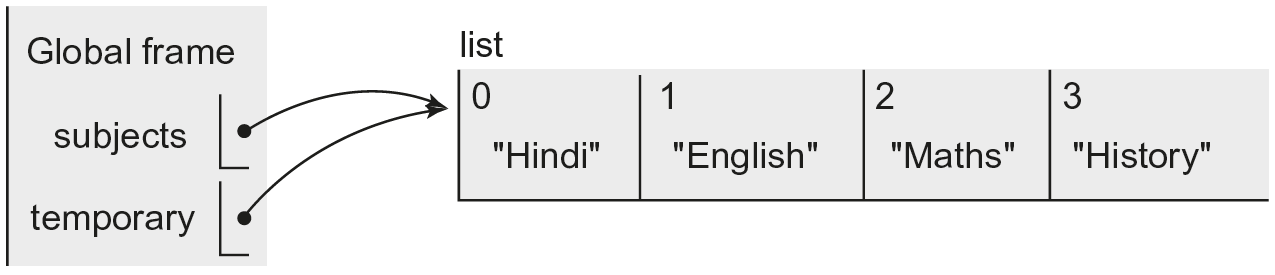
\includegraphics{3.png}

    \begin{Verbatim}[commandchars=\\\{\}]
{\color{incolor}In [{\color{incolor}129}]:} \PY{n}{temporary}\PY{p}{[}\PY{l+m+mi}{0}\PY{p}{]} \PY{o}{=} \PY{l+s+s1}{\PYZsq{}}\PY{l+s+s1}{Sanskrit}\PY{l+s+s1}{\PYZsq{}}
          \PY{n+nb}{print}\PY{p}{(}\PY{n}{temporary}\PY{p}{)}
          \PY{n+nb}{print}\PY{p}{(}\PY{n}{subjects}\PY{p}{)}
\end{Verbatim}


    \begin{Verbatim}[commandchars=\\\{\}]
['Sanskrit', 'English', 'Maths', 'History']
['Sanskrit', 'English', 'Maths', 'History']

    \end{Verbatim}

    \begin{Verbatim}[commandchars=\\\{\}]
{\color{incolor}In [{\color{incolor}130}]:} \PY{n}{subjectCodes} \PY{o}{=} \PY{p}{[}\PY{p}{[}\PY{l+s+s1}{\PYZsq{}}\PY{l+s+s1}{Sanskrit}\PY{l+s+s1}{\PYZsq{}}\PY{p}{,} \PY{l+m+mi}{43}\PY{p}{]}\PY{p}{,} \PY{p}{[}\PY{l+s+s1}{\PYZsq{}}\PY{l+s+s1}{English}\PY{l+s+s1}{\PYZsq{}}\PY{p}{,} \PY{l+m+mi}{85}\PY{p}{]} \PY{p}{,} \PY{p}{[}\PY{l+s+s1}{\PYZsq{}}\PY{l+s+s1}{Maths}\PY{l+s+s1}{\PYZsq{}}\PY{p}{,} \PY{l+m+mi}{65}\PY{p}{]}\PY{p}{,} \PY{p}{[}\PY{l+s+s1}{\PYZsq{}}\PY{l+s+s1}{History}\PY{l+s+s1}{\PYZsq{}}\PY{p}{,} \PY{l+m+mi}{36}\PY{p}{]}\PY{p}{]}
          \PY{n}{subjectCodes}\PY{p}{[}\PY{l+m+mi}{1}\PY{p}{]}
\end{Verbatim}


\begin{Verbatim}[commandchars=\\\{\}]
{\color{outcolor}Out[{\color{outcolor}130}]:} ['English', 85]
\end{Verbatim}
            
    \begin{Verbatim}[commandchars=\\\{\}]
{\color{incolor}In [{\color{incolor}131}]:} \PY{n+nb}{print}\PY{p}{(}\PY{n}{subjectCodes}\PY{p}{[}\PY{l+m+mi}{1}\PY{p}{]}\PY{p}{[}\PY{l+m+mi}{0}\PY{p}{]}\PY{p}{,}\PY{n}{subjectCodes}\PY{p}{[}\PY{l+m+mi}{1}\PY{p}{]}\PY{p}{[}\PY{l+m+mi}{1}\PY{p}{]}\PY{p}{)}
\end{Verbatim}


    \begin{Verbatim}[commandchars=\\\{\}]
English 85

    \end{Verbatim}

    \subsubsection{ Heterogeneous List }\label{heterogeneous-list}

    \begin{Verbatim}[commandchars=\\\{\}]
{\color{incolor}In [{\color{incolor}132}]:} \PY{n}{details} \PY{o}{=} \PY{p}{[}\PY{l+s+s1}{\PYZsq{}}\PY{l+s+s1}{Megha Verma}\PY{l+s+s1}{\PYZsq{}}\PY{p}{,} \PY{l+s+s1}{\PYZsq{}}\PY{l+s+s1}{C\PYZhy{}55, Raj Nagar, Pitam Pura, Delhi \PYZhy{} 110034}\PY{l+s+s1}{\PYZsq{}}\PY{p}{,} \PY{l+m+mi}{9876543210}\PY{p}{]}
\end{Verbatim}


    \subsection{ List Operations }\label{list-operations}

    \begin{Verbatim}[commandchars=\\\{\}]
{\color{incolor}In [{\color{incolor}156}]:} \PY{n}{list1} \PY{o}{=} \PY{p}{[}\PY{l+s+s1}{\PYZsq{}}\PY{l+s+s1}{Red}\PY{l+s+s1}{\PYZsq{}}\PY{p}{,} \PY{l+s+s1}{\PYZsq{}}\PY{l+s+s1}{Green}\PY{l+s+s1}{\PYZsq{}}\PY{p}{]}
          \PY{n}{list2} \PY{o}{=} \PY{p}{[}\PY{l+m+mi}{10}\PY{p}{,} \PY{l+m+mi}{20}\PY{p}{,} \PY{l+m+mi}{30}\PY{p}{]}
\end{Verbatim}


    \subsubsection{ Multiple Operator * }\label{multiple-operator}

    \begin{Verbatim}[commandchars=\\\{\}]
{\color{incolor}In [{\color{incolor}157}]:} \PY{n}{list2} \PY{o}{*} \PY{l+m+mi}{2}
\end{Verbatim}


\begin{Verbatim}[commandchars=\\\{\}]
{\color{outcolor}Out[{\color{outcolor}157}]:} [10, 20, 30, 10, 20, 30]
\end{Verbatim}
            
    \subsubsection{ Concatenation Operator + }\label{concatenation-operator}

    \begin{Verbatim}[commandchars=\\\{\}]
{\color{incolor}In [{\color{incolor}158}]:} \PY{n}{list1} \PY{o}{=} \PY{n}{list1} \PY{o}{+} \PY{p}{[}\PY{l+s+s1}{\PYZsq{}}\PY{l+s+s1}{Blue}\PY{l+s+s1}{\PYZsq{}}\PY{p}{]}
          \PY{n}{list1}
\end{Verbatim}


\begin{Verbatim}[commandchars=\\\{\}]
{\color{outcolor}Out[{\color{outcolor}158}]:} ['Red', 'Green', 'Blue']
\end{Verbatim}
            
    \subsubsection{ Length Operator len }\label{length-operator-len}

    \begin{Verbatim}[commandchars=\\\{\}]
{\color{incolor}In [{\color{incolor}159}]:} \PY{n+nb}{len}\PY{p}{(}\PY{n}{list1}\PY{p}{)}
\end{Verbatim}


\begin{Verbatim}[commandchars=\\\{\}]
{\color{outcolor}Out[{\color{outcolor}159}]:} 3
\end{Verbatim}
            
    \subsubsection{ Indexing \& Slicing }\label{indexing-slicing}

    \begin{Verbatim}[commandchars=\\\{\}]
{\color{incolor}In [{\color{incolor}160}]:} \PY{n}{list2}\PY{p}{[}\PY{o}{\PYZhy{}}\PY{l+m+mi}{1}\PY{p}{]}
\end{Verbatim}


\begin{Verbatim}[commandchars=\\\{\}]
{\color{outcolor}Out[{\color{outcolor}160}]:} 30
\end{Verbatim}
            
    \begin{Verbatim}[commandchars=\\\{\}]
{\color{incolor}In [{\color{incolor}161}]:} \PY{n}{list2}\PY{p}{[}\PY{l+m+mi}{0}\PY{p}{:}\PY{l+m+mi}{2}\PY{p}{]}
\end{Verbatim}


\begin{Verbatim}[commandchars=\\\{\}]
{\color{outcolor}Out[{\color{outcolor}161}]:} [10, 20]
\end{Verbatim}
            
    \begin{Verbatim}[commandchars=\\\{\}]
{\color{incolor}In [{\color{incolor}162}]:} \PY{n}{list2}\PY{p}{[}\PY{l+m+mi}{0}\PY{p}{:}\PY{l+m+mi}{3}\PY{p}{:}\PY{l+m+mi}{2}\PY{p}{]}
\end{Verbatim}


\begin{Verbatim}[commandchars=\\\{\}]
{\color{outcolor}Out[{\color{outcolor}162}]:} [10, 30]
\end{Verbatim}
            
    \subsubsection{ Function min \& max }\label{function-min-max}

    \begin{Verbatim}[commandchars=\\\{\}]
{\color{incolor}In [{\color{incolor}163}]:} \PY{n+nb}{min}\PY{p}{(}\PY{n}{list2}\PY{p}{)}
\end{Verbatim}


\begin{Verbatim}[commandchars=\\\{\}]
{\color{outcolor}Out[{\color{outcolor}163}]:} 10
\end{Verbatim}
            
    \begin{Verbatim}[commandchars=\\\{\}]
{\color{incolor}In [{\color{incolor}164}]:} \PY{n+nb}{max}\PY{p}{(}\PY{n}{list1}\PY{p}{)}
\end{Verbatim}


\begin{Verbatim}[commandchars=\\\{\}]
{\color{outcolor}Out[{\color{outcolor}164}]:} 'Red'
\end{Verbatim}
            
    \subsubsection{ Function sum }\label{function-sum}

    \begin{Verbatim}[commandchars=\\\{\}]
{\color{incolor}In [{\color{incolor}165}]:} \PY{n+nb}{sum}\PY{p}{(}\PY{n}{list2}\PY{p}{)}
\end{Verbatim}


\begin{Verbatim}[commandchars=\\\{\}]
{\color{outcolor}Out[{\color{outcolor}165}]:} 60
\end{Verbatim}
            
    \subsubsection{ Membership Operator: in }\label{membership-operator-in}

    \begin{Verbatim}[commandchars=\\\{\}]
{\color{incolor}In [{\color{incolor}166}]:} \PY{l+m+mi}{40} \PY{o+ow}{in} \PY{n}{list2}
\end{Verbatim}


\begin{Verbatim}[commandchars=\\\{\}]
{\color{outcolor}Out[{\color{outcolor}166}]:} False
\end{Verbatim}
            
    \begin{Verbatim}[commandchars=\\\{\}]
{\color{incolor}In [{\color{incolor}167}]:} \PY{n}{students} \PY{o}{=} \PY{p}{[}\PY{l+s+s1}{\PYZsq{}}\PY{l+s+s1}{Ram}\PY{l+s+s1}{\PYZsq{}}\PY{p}{,} \PY{l+s+s1}{\PYZsq{}}\PY{l+s+s1}{Shyam}\PY{l+s+s1}{\PYZsq{}}\PY{p}{,} \PY{l+s+s1}{\PYZsq{}}\PY{l+s+s1}{Gita}\PY{l+s+s1}{\PYZsq{}}\PY{p}{,} \PY{l+s+s1}{\PYZsq{}}\PY{l+s+s1}{Sita}\PY{l+s+s1}{\PYZsq{}}\PY{p}{]}
          \PY{k}{for} \PY{n}{name} \PY{o+ow}{in} \PY{n}{students}\PY{p}{:}
              \PY{n+nb}{print}\PY{p}{(}\PY{n}{name}\PY{p}{)}
\end{Verbatim}


    \begin{Verbatim}[commandchars=\\\{\}]
Ram
Shyam
Gita
Sita

    \end{Verbatim}

    \subsubsection{ Function list }\label{function-list}

\begin{itemize}
\tightlist
\item
  The function list takes a sequence as an argument and returns a list.
\end{itemize}

    \begin{Verbatim}[commandchars=\\\{\}]
{\color{incolor}In [{\color{incolor}168}]:} \PY{n}{vowels} \PY{o}{=} \PY{l+s+s1}{\PYZsq{}}\PY{l+s+s1}{aeiou}\PY{l+s+s1}{\PYZsq{}}
          \PY{n+nb}{list}\PY{p}{(}\PY{n}{vowels}\PY{p}{)}
\end{Verbatim}


\begin{Verbatim}[commandchars=\\\{\}]
{\color{outcolor}Out[{\color{outcolor}168}]:} ['a', 'e', 'i', 'o', 'u']
\end{Verbatim}
            
    \subsection{\texorpdfstring{ \textbf{Built-in Functions on Lists}
}{ Built-in Functions on Lists }}\label{built-in-functions-on-lists}

    \subsubsection{ Function append }\label{function-append}

\begin{itemize}
\tightlist
\item
  The function append insert the object passed to it at the end of the
  list.
\end{itemize}

    \begin{Verbatim}[commandchars=\\\{\}]
{\color{incolor}In [{\color{incolor}170}]:} \PY{n}{a} \PY{o}{=} \PY{p}{[}\PY{l+m+mi}{10}\PY{p}{,} \PY{l+m+mi}{20}\PY{p}{,} \PY{l+m+mi}{30}\PY{p}{,} \PY{l+m+mi}{40}\PY{p}{]}
          \PY{n}{a}\PY{o}{.}\PY{n}{append}\PY{p}{(}\PY{l+m+mi}{35}\PY{p}{)}
          \PY{n+nb}{print}\PY{p}{(}\PY{n}{a}\PY{p}{)}
\end{Verbatim}


    \begin{Verbatim}[commandchars=\\\{\}]
[10, 20, 30, 40, 35]

    \end{Verbatim}

    \subsubsection{ Function extend }\label{function-extend}

\begin{itemize}
\tightlist
\item
  The function extend accepts a sequence as an argument and puts the
  elements of the sequence at the end of the list.
\end{itemize}

    \begin{Verbatim}[commandchars=\\\{\}]
{\color{incolor}In [{\color{incolor}171}]:} \PY{n}{a} \PY{o}{=} \PY{p}{[}\PY{l+m+mi}{10}\PY{p}{,} \PY{l+m+mi}{20}\PY{p}{,} \PY{l+m+mi}{30}\PY{p}{]}
          \PY{n}{a}\PY{o}{.}\PY{n}{extend}\PY{p}{(}\PY{p}{[}\PY{l+m+mi}{35}\PY{p}{,}\PY{l+m+mi}{40}\PY{p}{]}\PY{p}{)}
          \PY{n+nb}{print}\PY{p}{(}\PY{n}{a}\PY{p}{)}
\end{Verbatim}


    \begin{Verbatim}[commandchars=\\\{\}]
[10, 20, 30, 35, 40]

    \end{Verbatim}

    \subsubsection{ Function:count }\label{functioncount}

\begin{itemize}
\tightlist
\item
  The function count returns the count of the number of times the object
  passed as an argument appears in the list.
\end{itemize}

    \begin{Verbatim}[commandchars=\\\{\}]
{\color{incolor}In [{\color{incolor}172}]:} \PY{n}{a} \PY{o}{=} \PY{p}{[}\PY{l+m+mi}{10}\PY{p}{,} \PY{l+m+mi}{20}\PY{p}{,} \PY{l+m+mi}{30}\PY{p}{,} \PY{l+m+mi}{10}\PY{p}{,} \PY{l+m+mi}{50}\PY{p}{,} \PY{l+m+mi}{20}\PY{p}{,} \PY{l+m+mi}{60}\PY{p}{,} \PY{l+m+mi}{20}\PY{p}{,} \PY{l+m+mi}{30}\PY{p}{,} \PY{l+m+mi}{55}\PY{p}{]}
          \PY{n+nb}{print}\PY{p}{(}\PY{n}{a}\PY{o}{.}\PY{n}{count}\PY{p}{(}\PY{l+m+mi}{20}\PY{p}{)}\PY{p}{)}
\end{Verbatim}


    \begin{Verbatim}[commandchars=\\\{\}]
3

    \end{Verbatim}

    \subsubsection{ Function pop }\label{function-pop}

\begin{itemize}
\tightlist
\item
  The function pop returns the element from the list whose index is
  passed as an argument, while removing it from the list.
\end{itemize}

    \begin{Verbatim}[commandchars=\\\{\}]
{\color{incolor}In [{\color{incolor}173}]:} \PY{n}{a} \PY{o}{=} \PY{p}{[}\PY{l+m+mi}{10}\PY{p}{,} \PY{l+m+mi}{20}\PY{p}{,} \PY{l+m+mi}{30}\PY{p}{,} \PY{l+m+mi}{10}\PY{p}{,} \PY{l+m+mi}{50}\PY{p}{,} \PY{l+m+mi}{20}\PY{p}{,} \PY{l+m+mi}{60}\PY{p}{,} \PY{l+m+mi}{20}\PY{p}{,} \PY{l+m+mi}{30}\PY{p}{,} \PY{l+m+mi}{55}\PY{p}{]}
          \PY{n}{a}\PY{o}{.}\PY{n}{pop}\PY{p}{(}\PY{l+m+mi}{3}\PY{p}{)}
          \PY{n+nb}{print}\PY{p}{(}\PY{n}{a}\PY{p}{)}
\end{Verbatim}


    \begin{Verbatim}[commandchars=\\\{\}]
[10, 20, 30, 50, 20, 60, 20, 30, 55]

    \end{Verbatim}

    \subsubsection{ Function remove }\label{function-remove}

\begin{itemize}
\tightlist
\item
  The function remove takes the value to be removed from the list as an
  argument, and removes the first occurrence of that value from the
  list.
\end{itemize}

    \begin{Verbatim}[commandchars=\\\{\}]
{\color{incolor}In [{\color{incolor}174}]:} \PY{n}{a}\PY{o}{.}\PY{n}{remove}\PY{p}{(}\PY{l+m+mi}{20}\PY{p}{)}
          \PY{n+nb}{print}\PY{p}{(}\PY{n}{a}\PY{p}{)}
\end{Verbatim}


    \begin{Verbatim}[commandchars=\\\{\}]
[10, 30, 50, 20, 60, 20, 30, 55]

    \end{Verbatim}

    \subsubsection{ del Operator }\label{del-operator}

\begin{itemize}
\tightlist
\item
  The del operator is used to remove a subsequence of elements
  (start:end:increment) from a list.
\end{itemize}

    \begin{Verbatim}[commandchars=\\\{\}]
{\color{incolor}In [{\color{incolor}175}]:} \PY{n}{a} \PY{o}{=} \PY{p}{[}\PY{l+m+mi}{10}\PY{p}{,} \PY{l+m+mi}{20}\PY{p}{,} \PY{l+m+mi}{30}\PY{p}{,} \PY{l+m+mi}{20}\PY{p}{,} \PY{l+m+mi}{60}\PY{p}{,} \PY{l+m+mi}{20}\PY{p}{,} \PY{l+m+mi}{30}\PY{p}{,} \PY{l+m+mi}{55}\PY{p}{]}
          \PY{k}{del} \PY{n}{a}\PY{p}{[}\PY{l+m+mi}{2}\PY{p}{:}\PY{l+m+mi}{6}\PY{p}{:}\PY{l+m+mi}{3}\PY{p}{]}
          \PY{n+nb}{print}\PY{p}{(}\PY{n}{a}\PY{p}{)}
\end{Verbatim}


    \begin{Verbatim}[commandchars=\\\{\}]
[10, 20, 20, 60, 30, 55]

    \end{Verbatim}

    \subsubsection{ Function insert }\label{function-insert}

\begin{itemize}
\tightlist
\item
  The insert function can be used to insert an object at a specified
  index. This function takes two arguments: the index where an object is
  to be inserted and the object itself.
\end{itemize}

    \begin{Verbatim}[commandchars=\\\{\}]
{\color{incolor}In [{\color{incolor}176}]:} \PY{n}{names} \PY{o}{=} \PY{p}{[}\PY{l+s+s1}{\PYZsq{}}\PY{l+s+s1}{Ram}\PY{l+s+s1}{\PYZsq{}}\PY{p}{,} \PY{l+s+s1}{\PYZsq{}}\PY{l+s+s1}{Sita}\PY{l+s+s1}{\PYZsq{}}\PY{p}{,} \PY{l+s+s1}{\PYZsq{}}\PY{l+s+s1}{Gita}\PY{l+s+s1}{\PYZsq{}}\PY{p}{,} \PY{l+s+s1}{\PYZsq{}}\PY{l+s+s1}{Sita}\PY{l+s+s1}{\PYZsq{}}\PY{p}{]}
          \PY{n}{names}\PY{o}{.}\PY{n}{insert}\PY{p}{(}\PY{l+m+mi}{2}\PY{p}{,} \PY{l+s+s1}{\PYZsq{}}\PY{l+s+s1}{Shyam}\PY{l+s+s1}{\PYZsq{}}\PY{p}{)}
          \PY{n+nb}{print}\PY{p}{(}\PY{n}{names}\PY{p}{)}
\end{Verbatim}


    \begin{Verbatim}[commandchars=\\\{\}]
['Ram', 'Sita', 'Shyam', 'Gita', 'Sita']

    \end{Verbatim}

    \subsubsection{ Function reverse }\label{function-reverse}

\begin{itemize}
\tightlist
\item
  The function reverse reverses the order of the elements in a list.
\end{itemize}

    \begin{Verbatim}[commandchars=\\\{\}]
{\color{incolor}In [{\color{incolor}178}]:} \PY{n}{names} \PY{o}{=} \PY{p}{[}\PY{l+s+s1}{\PYZsq{}}\PY{l+s+s1}{Ram}\PY{l+s+s1}{\PYZsq{}}\PY{p}{,} \PY{l+s+s1}{\PYZsq{}}\PY{l+s+s1}{Sita}\PY{l+s+s1}{\PYZsq{}}\PY{p}{,} \PY{l+s+s1}{\PYZsq{}}\PY{l+s+s1}{Sita}\PY{l+s+s1}{\PYZsq{}}\PY{p}{,} \PY{l+s+s1}{\PYZsq{}}\PY{l+s+s1}{Anya}\PY{l+s+s1}{\PYZsq{}}\PY{p}{]}
          \PY{n}{names}\PY{o}{.}\PY{n}{reverse}\PY{p}{(}\PY{p}{)}
          \PY{n+nb}{print}\PY{p}{(}\PY{n}{names}\PY{p}{)}
\end{Verbatim}


    \begin{Verbatim}[commandchars=\\\{\}]
['Anya', 'Sita', 'Sita', 'Ram']

    \end{Verbatim}

    \subsubsection{ Function sort }\label{function-sort}

\begin{itemize}
\tightlist
\item
  The function sort can be used to arrange the elements in a list in
  ascending order.
\end{itemize}

    \begin{Verbatim}[commandchars=\\\{\}]
{\color{incolor}In [{\color{incolor}179}]:} \PY{n}{names} \PY{o}{=} \PY{p}{[}\PY{l+s+s1}{\PYZsq{}}\PY{l+s+s1}{Ram}\PY{l+s+s1}{\PYZsq{}}\PY{p}{,} \PY{l+s+s1}{\PYZsq{}}\PY{l+s+s1}{Sita}\PY{l+s+s1}{\PYZsq{}}\PY{p}{,} \PY{l+s+s1}{\PYZsq{}}\PY{l+s+s1}{Sita}\PY{l+s+s1}{\PYZsq{}}\PY{p}{,} \PY{l+s+s1}{\PYZsq{}}\PY{l+s+s1}{Anya}\PY{l+s+s1}{\PYZsq{}}\PY{p}{]}
          \PY{n}{names}\PY{o}{.}\PY{n}{sort}\PY{p}{(}\PY{p}{)}
          \PY{n+nb}{print}\PY{p}{(}\PY{n}{names}\PY{p}{)}
\end{Verbatim}


    \begin{Verbatim}[commandchars=\\\{\}]
['Anya', 'Ram', 'Sita', 'Sita']

    \end{Verbatim}

    \begin{Verbatim}[commandchars=\\\{\}]
{\color{incolor}In [{\color{incolor}180}]:} \PY{n}{names} \PY{o}{=} \PY{p}{[}\PY{l+s+s1}{\PYZsq{}}\PY{l+s+s1}{Ram}\PY{l+s+s1}{\PYZsq{}}\PY{p}{,} \PY{l+s+s1}{\PYZsq{}}\PY{l+s+s1}{Sita}\PY{l+s+s1}{\PYZsq{}}\PY{p}{,} \PY{l+s+s1}{\PYZsq{}}\PY{l+s+s1}{Sita}\PY{l+s+s1}{\PYZsq{}}\PY{p}{,} \PY{l+s+s1}{\PYZsq{}}\PY{l+s+s1}{Anya}\PY{l+s+s1}{\PYZsq{}}\PY{p}{]}
          \PY{n}{names}\PY{o}{.}\PY{n}{sort}\PY{p}{(}\PY{n}{reverse} \PY{o}{=} \PY{k+kc}{True}\PY{p}{)}
          \PY{n+nb}{print}\PY{p}{(}\PY{n}{names}\PY{p}{)}
\end{Verbatim}


    \begin{Verbatim}[commandchars=\\\{\}]
['Sita', 'Sita', 'Ram', 'Anya']

    \end{Verbatim}

    \subsection{ Problem: List of n terms of fibonacci series
}\label{problem-list-of-n-terms-of-fibonacci-series}

    \begin{Verbatim}[commandchars=\\\{\}]
{\color{incolor}In [{\color{incolor}3}]:} \PY{k}{def} \PY{n+nf}{fib}\PY{p}{(}\PY{n}{n}\PY{p}{)}\PY{p}{:}
            \PY{l+s+sd}{\PYZsq{}\PYZsq{}\PYZsq{}}
        \PY{l+s+sd}{    Objective: To return list of n terms of fibonacci series.}
        \PY{l+s+sd}{    Input Parameter: n \PYZhy{} numeric}
        \PY{l+s+sd}{    Return Value: numeric}
        \PY{l+s+sd}{    \PYZsq{}\PYZsq{}\PYZsq{}}
            \PY{l+s+sd}{\PYZsq{}\PYZsq{}\PYZsq{}}
        \PY{l+s+sd}{    Approach:}
        \PY{l+s+sd}{        Create a list with 0 and 1 as first two numbers of fibonacci series.}
        \PY{l+s+sd}{        For each subsequent number, append sum of previous two numbers to}
        \PY{l+s+sd}{        the list.}
        \PY{l+s+sd}{    \PYZsq{}\PYZsq{}\PYZsq{}}
            \PY{k}{if} \PY{n}{n} \PY{o}{\PYZlt{}}\PY{o}{=}\PY{l+m+mi}{0}\PY{p}{:}
                \PY{k}{return} \PY{k+kc}{None}
            \PY{k}{elif} \PY{n}{n} \PY{o}{==}\PY{l+m+mi}{1}\PY{p}{:}
                \PY{k}{return} \PY{p}{[}\PY{l+m+mi}{0}\PY{p}{]}
            \PY{k}{elif} \PY{n}{n} \PY{o}{==} \PY{l+m+mi}{2}\PY{p}{:}
                \PY{k}{return} \PY{p}{[}\PY{l+m+mi}{0}\PY{p}{,} \PY{l+m+mi}{1}\PY{p}{]}
            \PY{k}{else}\PY{p}{:}
                \PY{n}{resList} \PY{o}{=} \PY{p}{[}\PY{p}{]}
                \PY{n}{a}\PY{p}{,} \PY{n}{b} \PY{o}{=} \PY{l+m+mi}{0}\PY{p}{,} \PY{l+m+mi}{1}
                \PY{n}{resList}\PY{o}{.}\PY{n}{append}\PY{p}{(}\PY{n}{a}\PY{p}{)}
                \PY{n}{resList}\PY{o}{.}\PY{n}{append}\PY{p}{(}\PY{n}{b}\PY{p}{)}
                \PY{n}{count} \PY{o}{=} \PY{l+m+mi}{3}
                \PY{k}{while}  \PY{n}{count} \PY{o}{\PYZlt{}}\PY{o}{=} \PY{n}{n}\PY{p}{:}
                    \PY{n}{c} \PY{o}{=} \PY{n}{a} \PY{o}{+} \PY{n}{b}
                    \PY{n}{resList}\PY{o}{.}\PY{n}{append}\PY{p}{(}\PY{n}{c}\PY{p}{)}
                    \PY{n}{a} \PY{o}{=} \PY{n}{b}
                    \PY{n}{b} \PY{o}{=} \PY{n}{c}
                    \PY{n}{count} \PY{o}{+}\PY{o}{=} \PY{l+m+mi}{1}
                \PY{k}{return} \PY{n}{resList}
        
        \PY{k}{def} \PY{n+nf}{main}\PY{p}{(}\PY{p}{)}\PY{p}{:}
            \PY{l+s+sd}{\PYZsq{}\PYZsq{}\PYZsq{}}
        \PY{l+s+sd}{    Objective: To print n terms of fibonacci series based on user input}
        \PY{l+s+sd}{    Input Parameter: None}
        \PY{l+s+sd}{    Return Value: None}
        \PY{l+s+sd}{    \PYZsq{}\PYZsq{}\PYZsq{}}
            \PY{n}{num} \PY{o}{=} \PY{n+nb}{int}\PY{p}{(}\PY{n+nb}{input}\PY{p}{(}\PY{l+s+s1}{\PYZsq{}}\PY{l+s+s1}{Enter no. of terms:}\PY{l+s+s1}{\PYZsq{}}\PY{p}{)}\PY{p}{)}
            \PY{n}{result} \PY{o}{=} \PY{n}{fib}\PY{p}{(}\PY{n}{num}\PY{p}{)}
            \PY{n+nb}{print}\PY{p}{(}\PY{n}{result}\PY{p}{)}
        
        \PY{k}{if} \PY{n+nv+vm}{\PYZus{}\PYZus{}name\PYZus{}\PYZus{}} \PY{o}{==} \PY{l+s+s1}{\PYZsq{}}\PY{l+s+s1}{\PYZus{}\PYZus{}main\PYZus{}\PYZus{}}\PY{l+s+s1}{\PYZsq{}}\PY{p}{:}
            \PY{n}{main}\PY{p}{(}\PY{p}{)}
\end{Verbatim}


    \begin{Verbatim}[commandchars=\\\{\}]
Enter no. of terms:6
[0, 1, 1, 2, 3, 5]

    \end{Verbatim}


    % Add a bibliography block to the postdoc
    
    
    
    \end{document}
